%!TEX root = ../document.tex
\chapter{Project Scope}

\section{Stakeholders}

Terrafugia, AeroMobil, PAL-V One, Moller International, Zee.Aero and Urban Aeronautics are among the few well-known names in this regard who are trying to make future Flying Cars real one day. Volkswagen, Toyota are the established mobile companies that have also been working on the concept of Flying Car. Besides, there are others like NASA, US military backed organisations and the Boeing company that are working on to bring up a flying car that can serve civilian as well rescue operations needs. The following picture is the stakeholder mapping.

\begin{figure}[H]
\centering
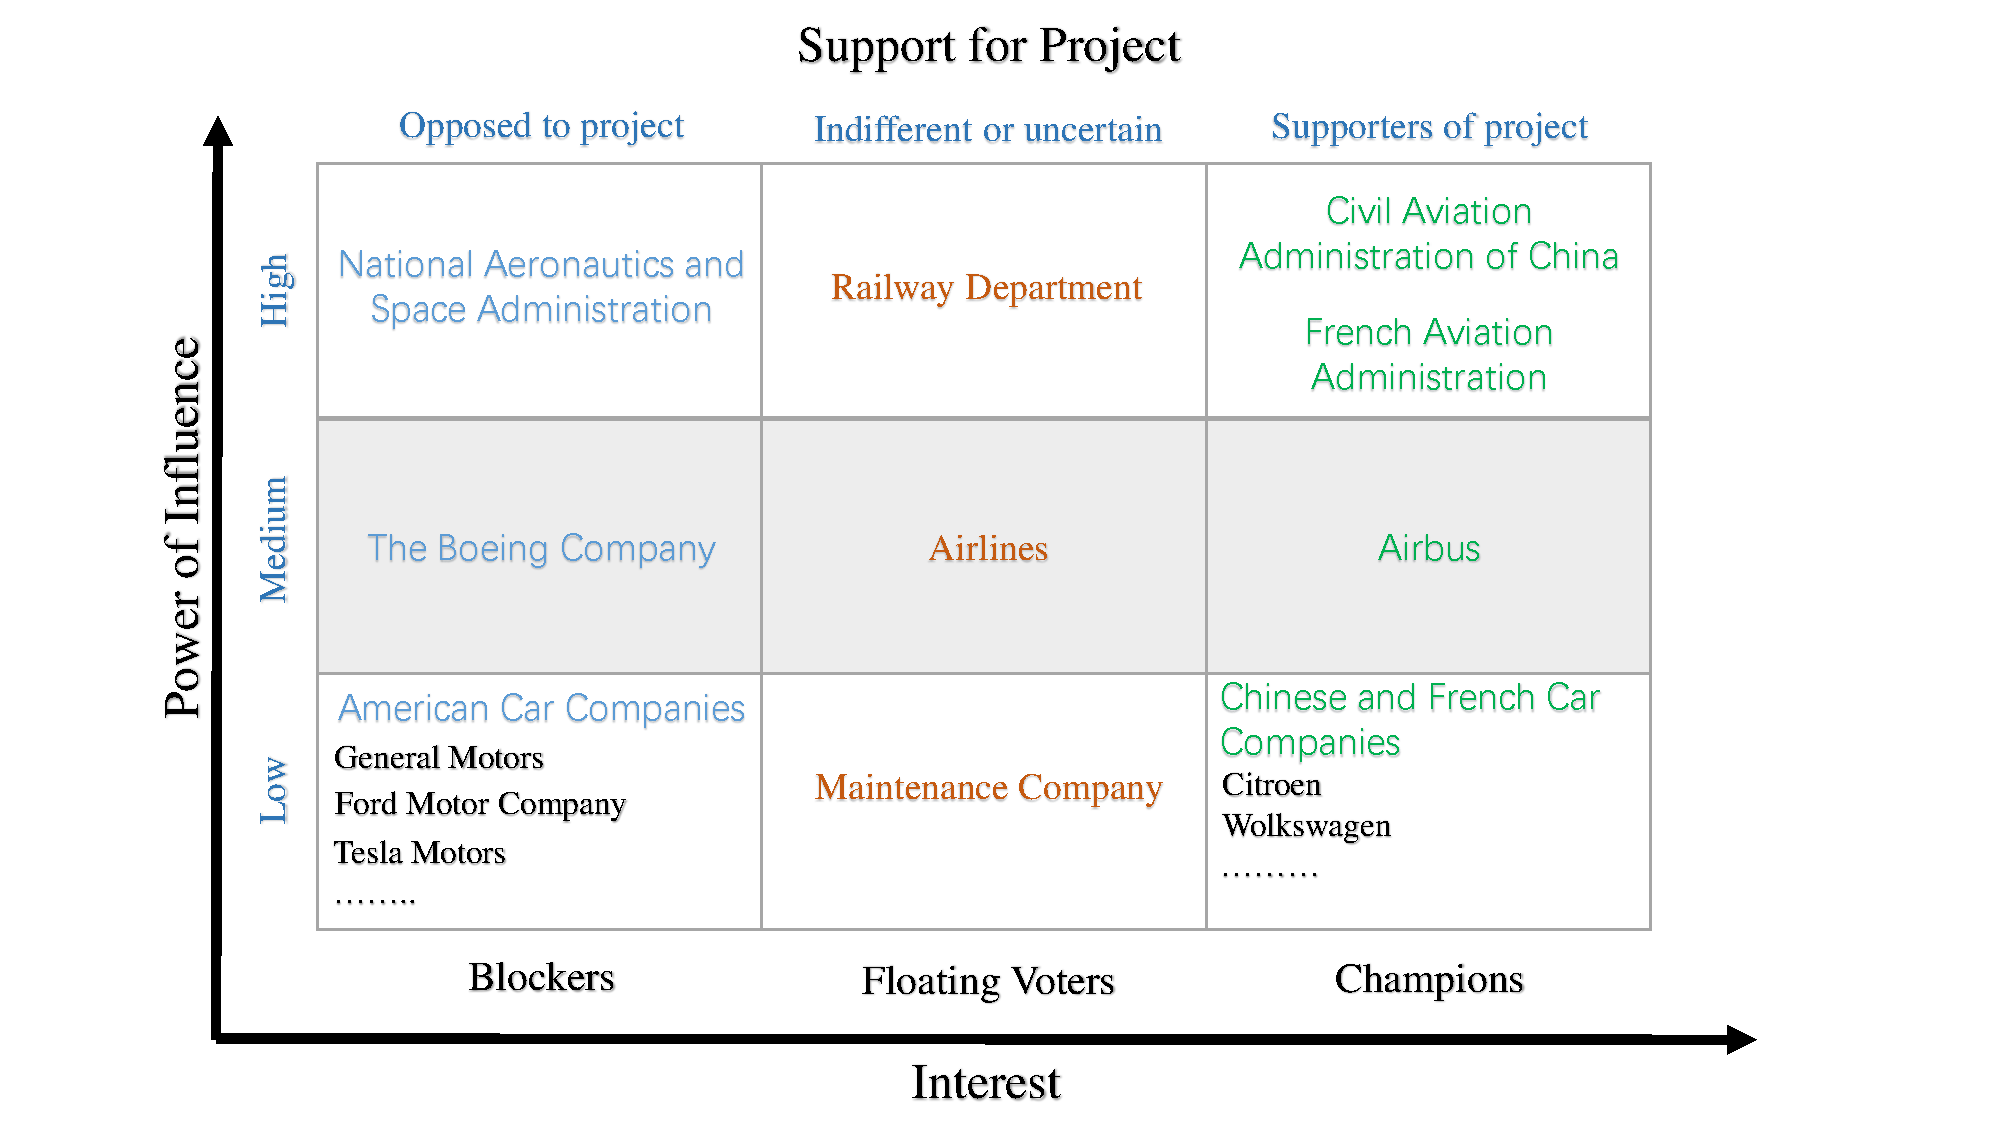
\includegraphics[width=14cm]{pic/stakeholders.pdf}
% \caption{stakeholders}
% \label{fig:stakeholders}
\end{figure}

\subsection{Project sponsor}

Civil Aviation Administration of China, the aviation authority under the Ministry of Transport of the People's Republic of China is the sponsor of this project, who aims at improving the whole situation of Chinese aviation and transportation.. It oversees civil aviation and investigates aviation accidents and incidents. As the aviation authority responsible for China, it concludes civil aviation agreements with other aviation authorities, including those of the Special administrative regions of China which are categorized as "special domestic".

\subsection{Project team members}

Companies Terrafugia, AeroMobil, PAL-V One and Zee.Aero are considered to be the major components of the project team along with the companies Citroen, Volkswagen and Airbus who provide the technical support aviatic and terrestrial.

\begin{enumerate}

\item \textbf{Terrafugia}

Terrafugia, founded by MIT Grads is a company that is expected to launch the Transition Model after testing to check meeting standards for air and road safety underlined by Federal Aviation Regulatory body.

The company has already intended to receive about 100 pre-orders on Transition mode after announcing launch in upcoming years. Besides the next generation model Terrafugia TF-X would also be developed with increased automation and scheduled for commercial availability after ten years post its debut in 2019 if it undergoes all tests successfully.

\item \textbf{Aeromobil}

Aeromobil, a company has come up with an upgraded prototype of flying car AeroMobil 3.0. After an initial test crash, AeroMobil 3.0 finally made a successful maiden flight in the last decade. The CEO Juraj Vaculik had suggested the company’s plans to launch the model commercially. The importance of meeting regulatory standards for a flying vehicle cannot be understated and thus it would not be surprising if there occurs further delay by a couple of years before the final launch. Besides, AeroMobil also plans to make a fully automated version of the prototype for increased safety and comfort standards.

\item \textbf{PALV}

PALV is a company from Netherlands that has developed a Personal Air And Land Vehicle Prototype PAL-V One that it claims can give experience of driving a sports car on road and at the same time like a flying bird in the sky giving a dimension of freedom by taking off from one island and landing to another, flying over  mountain ranges and rivers.

\item \textbf{Aero}

Aero, a small company inZhongguancun Science and Technology Park is working on to flying car concept to build up a VTOL machine. A patent filed by the company states that the VTOL car is capable of getting parked in a shopping mall. The project lead Ilan Kroo, an aeronautics professor and NASA scientist. The Aero has been designed in an arrangement that is called as ‘Canard wing’ wherein the payload area lies between front and rear set of wings.

\end{enumerate}

\subsection{Project customer}

The customer will originally be someone or some companies who have an interest or a gain upon a successful completion of the project. We will divide them into three parts.

First, several airlines such as China Southern Airlines and Air China. As the economic roars, the plane has sneaked into every inch of our transportation, this new concept “flying car” is possibly to lead a trend of new convenient method of transportation. Therefore the airlines may consider it as another type of aircraft. Furthermore , we could named it Boeing 797.

Second, as the flying car may serve as a powerful alternative and prioritized option of car in the future, by which the vehicles like private cars are potential to be replaced. Looking at the future development, the car companies such as BMW group and Toyota Motor Corporation are also supposed to renew their products, they launch am annual release of a new system, attend the annual conference and conduct academic research. Supposing that the flying cars will be gradually accepted by the public, it is high time for them to introduce this new product.

What’s more, the flying cars could attract individuals who are obsessed with cars or planes. The flying car is exactly a consummate combination which not only offers countless opportunities to maximize efficiency, but also spice up the journey on the road.


\section{Technology}

\subsection{Modeling}

In terms of the model of the flying car, the project will select the most compatible one among several models created by the software CATIA. The main function and part are same, however, we are about to simplify the model into an optimization problem and find the best. Optimization problems are often multi-modal; that is, they possess multiple good solutions. They could all be globally good (same cost function value) or there could be a mix of globally good and locally good solutions. Obtaining all (or at least some of) the multiple solutions is the goal of a multi-modal optimizer. 

Classical optimization techniques due to their iterative approach do not perform satisfactorily when they are used to obtain multiple solutions, since it is not guaranteed that different solutions will be obtained even with different starting points in multiple runs of the algorithm. Evolutionary algorithms, however, are a very popular approach to obtain multiple solutions in a multi-modal optimization task.

\begin{figure}[H]
\centering
\begin{minipage}[t]{0.48\textwidth}
\centering
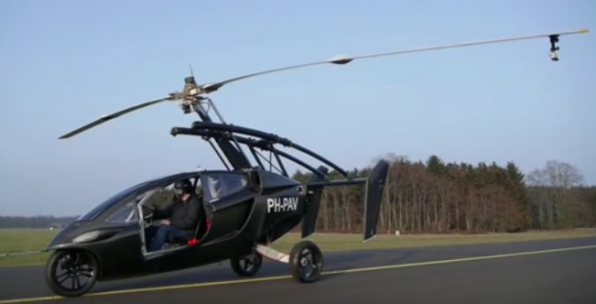
\includegraphics[width=7.5cm]{pic/m3.png}
\end{minipage}
\begin{minipage}[t]{0.48\textwidth}
\centering
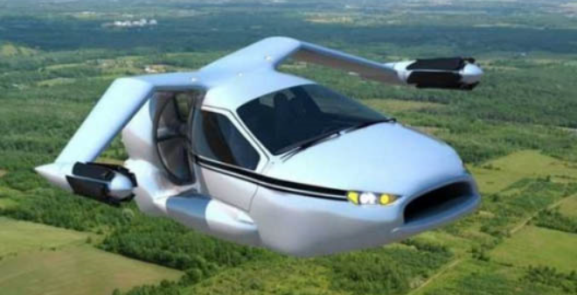
\includegraphics[width=7.5cm]{pic/m2.png}
\end{minipage}
\\[5mm]
\begin{minipage}[t]{0.48\textwidth}
\centering
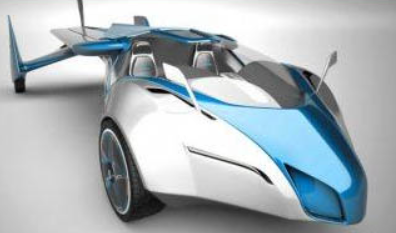
\includegraphics[width=7.5cm]{pic/m1.png}
\end{minipage}
\begin{minipage}[t]{0.48\textwidth}
\centering
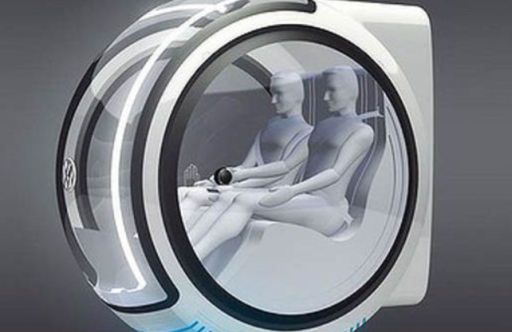
\includegraphics[width=7.5cm]{pic/m4.png}
\end{minipage}
\end{figure}

\subsection{Engine}

Ion engine will be the major component that generate the flying car. Ion thrusters use beams of ions (electrically charged atoms or molecules) to create thrust in accordance with momentum conservation. The method of accelerating the ions varies, but all designs take advantage of the charge/mass ratio of the ions. This ratio means that relatively small potential differences can create high exhaust velocities. This reduces the amount of reaction mass or propellant required, but increases the amount of specific power required compared to chemical rockets. Ion thrusters are therefore able to achieve high specific impulses. The drawback of the low thrust is low acceleration because the mass of the electric power unit directly correlates with the amount of power. This low thrust makes ion thrusters unsuited for launching spacecraft into orbit, but effective for in-space propulsion. 

They are categorized as either electrostatic or electromagnetic. The main difference is the method for accelerating the ions. Electrostatic ion thrusters use the Coulomb force and accelerate the ions in the direction of the electric field. Electromagnetic ion thrusters use the Lorentz force to move the ions. Therefore, this problem should also be solved.

\subsection{Material}

The composite materials and the alloy will compose the main materials of the flying cars, especially the composite material like Fibre-reinforced polymers(FPR).

FRP include carbon-fibre-reinforced polymer(CFRP) and glass-reinforced plastic(GRP). If classified by matrix then there are thermoplastic composites, short fibre thermoplastics, long fibre thermoplastics or long fibre-reinforced thermoplastics. There are numerous thermoset composites, including paper composite panels. Many advanced thermoset polymer matrix systems usually incorporate aramid fibre and carbon fibre in an epoxy resin matrix.

\subsection{Flight control system}

A conventional fixed-wing aircraft flight control system consists of flight control surfaces, the respective cockpit controls, connecting linkages, and the necessary operating mechanisms to control an aircraft's direction in flight. Aircraft engine controls are also considered as flight controls as they change speed.

The fundamentals of aircraft controls are explained in flight dynamics. This article centers on the operating mechanisms of the flight controls. Our flight control system are determined to imitate the technology of Airbus, and will be gradually transformed to an unmanned aerial vehicle(UAV), commonly known as a drone.

\subsection{Test-analysis}

The simulation of the flying car will use the method of Verification and Validation(V\&V).

Verification is the process of determining that a model implementation accurately represents the developer’s conceptual description of the model and the solution to the model.

Validation is the process of determining the degree to which a model is an accurate representation of the real world from the perspective of the intended uses of the model.

Verification and validation are processes that collect evidence of a model’s correctness or accuracy for a specific scenario; thus, V\&V cannot prove that a model is correct and accurate for all possible conditions and applications, but, rather, it can provide evidence that a model is sufficiently accurate. Therefore, the V\&V process is completed when sufficiency is reached.